\documentclass[1p]{elsarticle_modified}
%\bibliographystyle{elsarticle-num}

%\usepackage[colorlinks]{hyperref}
%\usepackage{abbrmath_seonhwa} %\Abb, \Ascr, \Acal ,\Abf, \Afrak
\usepackage{amsfonts}
\usepackage{amssymb}
\usepackage{amsmath}
\usepackage{amsthm}
\usepackage{scalefnt}
\usepackage{amsbsy}
\usepackage{kotex}
\usepackage{caption}
\usepackage{subfig}
\usepackage{color}
\usepackage{graphicx}
\usepackage{xcolor} %% white, black, red, green, blue, cyan, magenta, yellow
\usepackage{float}
\usepackage{setspace}
\usepackage{hyperref}

\usepackage{tikz}
\usetikzlibrary{arrows}

\usepackage{multirow}
\usepackage{array} % fixed length table
\usepackage{hhline}

%%%%%%%%%%%%%%%%%%%%%
\makeatletter
\renewcommand*\env@matrix[1][\arraystretch]{%
	\edef\arraystretch{#1}%
	\hskip -\arraycolsep
	\let\@ifnextchar\new@ifnextchar
	\array{*\c@MaxMatrixCols c}}
\makeatother %https://tex.stackexchange.com/questions/14071/how-can-i-increase-the-line-spacing-in-a-matrix
%%%%%%%%%%%%%%%

\usepackage[normalem]{ulem}

\newcommand{\msout}[1]{\ifmmode\text{\sout{\ensuremath{#1}}}\else\sout{#1}\fi}
%SOURCE: \msout is \stkout macro in https://tex.stackexchange.com/questions/20609/strikeout-in-math-mode

\newcommand{\cancel}[1]{
	\ifmmode
	{\color{red}\msout{#1}}
	\else
	{\color{red}\sout{#1}}
	\fi
}

\newcommand{\add}[1]{
	{\color{blue}\uwave{#1}}
}

\newcommand{\replace}[2]{
	\ifmmode
	{\color{red}\msout{#1}}{\color{blue}\uwave{#2}}
	\else
	{\color{red}\sout{#1}}{\color{blue}\uwave{#2}}
	\fi
}

\newcommand{\Sol}{\mathcal{S}} %segment
\newcommand{\D}{D} %diagram
\newcommand{\A}{\mathcal{A}} %arc


%%%%%%%%%%%%%%%%%%%%%%%%%%%%%5 test

\def\sl{\operatorname{\textup{SL}}(2,\Cbb)}
\def\psl{\operatorname{\textup{PSL}}(2,\Cbb)}
\def\quan{\mkern 1mu \triangleright \mkern 1mu}

\theoremstyle{definition}
\newtheorem{thm}{Theorem}[section]
\newtheorem{prop}[thm]{Proposition}
\newtheorem{lem}[thm]{Lemma}
\newtheorem{ques}[thm]{Question}
\newtheorem{cor}[thm]{Corollary}
\newtheorem{defn}[thm]{Definition}
\newtheorem{exam}[thm]{Example}
\newtheorem{rmk}[thm]{Remark}
\newtheorem{alg}[thm]{Algorithm}

\newcommand{\I}{\sqrt{-1}}
\begin{document}

%\begin{frontmatter}
%
%\title{Boundary parabolic representations of knots up to 8 crossings}
%
%%% Group authors per affiliation:
%\author{Yunhi Cho} 
%\address{Department of Mathematics, University of Seoul, Seoul, Korea}
%\ead{yhcho@uos.ac.kr}
%
%
%\author{Seonhwa Kim} %\fnref{s_kim}}
%\address{Center for Geometry and Physics, Institute for Basic Science, Pohang, 37673, Korea}
%\ead{ryeona17@ibs.re.kr}
%
%\author{Hyuk Kim}
%\address{Department of Mathematical Sciences, Seoul National University, Seoul 08826, Korea}
%\ead{hyukkim@snu.ac.kr}
%
%\author{Seokbeom Yoon}
%\address{Department of Mathematical Sciences, Seoul National University, Seoul, 08826,  Korea}
%\ead{sbyoon15@snu.ac.kr}
%
%\begin{abstract}
%We find all boundary parabolic representation of knots up to 8 crossings.
%
%\end{abstract}
%\begin{keyword}
%    \MSC[2010] 57M25 
%\end{keyword}
%
%\end{frontmatter}

%\linenumbers
%\tableofcontents
%
\newcommand\colored[1]{\textcolor{white}{\rule[-0.35ex]{0.8em}{1.4ex}}\kern-0.8em\color{red} #1}%
%\newcommand\colored[1]{\textcolor{white}{ #1}\kern-2.17ex	\textcolor{white}{ #1}\kern-1.81ex	\textcolor{white}{ #1}\kern-2.15ex\color{red}#1	}

{\Large $\underline{11a_{262}~(K11a_{262})}$}

\setlength{\tabcolsep}{10pt}
\renewcommand{\arraystretch}{1.6}
\vspace{1cm}\begin{tabular}{m{100pt}>{\centering\arraybackslash}m{274pt}}
\multirow{5}{120pt}{
	\centering
	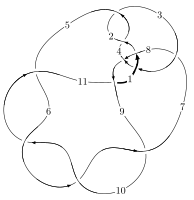
\includegraphics[width=112pt]{../../../GIT/diagram.site/Diagrams/png/511_11a_262.png}\\
\ \ \ A knot diagram\footnotemark}&
\allowdisplaybreaks
\textbf{Linearized knot diagam} \\
\cline{2-2}
 &
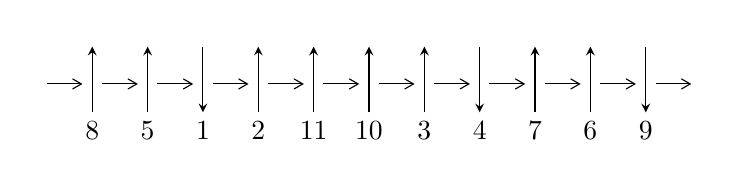
\begin{tikzpicture}[x=20pt, y=17pt]
	% nodes
	\node (C0) at (0, 0) {};
	\node (C1) at (1, 0) {};
	\node (C1U) at (1, +1) {};
	\node (C1D) at (1, -1) {8};

	\node (C2) at (2, 0) {};
	\node (C2U) at (2, +1) {};
	\node (C2D) at (2, -1) {5};

	\node (C3) at (3, 0) {};
	\node (C3U) at (3, +1) {};
	\node (C3D) at (3, -1) {1};

	\node (C4) at (4, 0) {};
	\node (C4U) at (4, +1) {};
	\node (C4D) at (4, -1) {2};

	\node (C5) at (5, 0) {};
	\node (C5U) at (5, +1) {};
	\node (C5D) at (5, -1) {11};

	\node (C6) at (6, 0) {};
	\node (C6U) at (6, +1) {};
	\node (C6D) at (6, -1) {10};

	\node (C7) at (7, 0) {};
	\node (C7U) at (7, +1) {};
	\node (C7D) at (7, -1) {3};

	\node (C8) at (8, 0) {};
	\node (C8U) at (8, +1) {};
	\node (C8D) at (8, -1) {4};

	\node (C9) at (9, 0) {};
	\node (C9U) at (9, +1) {};
	\node (C9D) at (9, -1) {7};

	\node (C10) at (10, 0) {};
	\node (C10U) at (10, +1) {};
	\node (C10D) at (10, -1) {6};

	\node (C11) at (11, 0) {};
	\node (C11U) at (11, +1) {};
	\node (C11D) at (11, -1) {9};
	\node (C12) at (12, 0) {};

	% arrows
	\draw[->,>={angle 60}]
	(C0) edge (C1) (C1) edge (C2) (C2) edge (C3) (C3) edge (C4) (C4) edge (C5) (C5) edge (C6) (C6) edge (C7) (C7) edge (C8) (C8) edge (C9) (C9) edge (C10) (C10) edge (C11) (C11) edge (C12) ;	\draw[->,>=stealth]
	(C1D) edge (C1U) (C2D) edge (C2U) (C3U) edge (C3D) (C4D) edge (C4U) (C5D) edge (C5U) (C6D) edge (C6U) (C7D) edge (C7U) (C8U) edge (C8D) (C9D) edge (C9U) (C10D) edge (C10U) (C11U) edge (C11D) ;
	\end{tikzpicture} \\
\hhline{~~} \\& 
\textbf{Solving Sequence} \\ \cline{2-2} 
 &
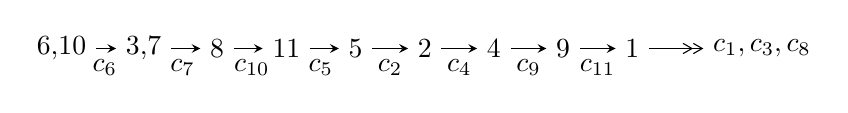
\begin{tikzpicture}[x=25pt, y=7pt]
	% node
	\node (A0) at (-1/8, 0) {6,10};
	\node (A1) at (17/16, 0) {3,7};
	\node (A2) at (17/8, 0) {8};
	\node (A3) at (25/8, 0) {11};
	\node (A4) at (33/8, 0) {5};
	\node (A5) at (41/8, 0) {2};
	\node (A6) at (49/8, 0) {4};
	\node (A7) at (57/8, 0) {9};
	\node (A8) at (65/8, 0) {1};
	\node (C1) at (1/2, -1) {$c_{6}$};
	\node (C2) at (13/8, -1) {$c_{7}$};
	\node (C3) at (21/8, -1) {$c_{10}$};
	\node (C4) at (29/8, -1) {$c_{5}$};
	\node (C5) at (37/8, -1) {$c_{2}$};
	\node (C6) at (45/8, -1) {$c_{4}$};
	\node (C7) at (53/8, -1) {$c_{9}$};
	\node (C8) at (61/8, -1) {$c_{11}$};
	\node (A9) at (10, 0) {$c_{1},c_{3},c_{8}$};

	% edge
	\draw[->,>=stealth]	
	(A0) edge (A1) (A1) edge (A2) (A2) edge (A3) (A3) edge (A4) (A4) edge (A5) (A5) edge (A6) (A6) edge (A7) (A7) edge (A8) ;
	\draw[->>,>={angle 60}]	
	(A8) edge (A9);
\end{tikzpicture} \\ 

\end{tabular} \\

\footnotetext{
The image of knot diagram is generated by the software ``\textbf{Draw programme}" developed by Andrew Bartholomew(\url{http://www.layer8.co.uk/maths/draw/index.htm\#Running-draw}), where we modified some parts for our purpose(\url{https://github.com/CATsTAILs/LinksPainter}).
}\phantom \\ \newline 
\centering \textbf{Ideals for irreducible components\footnotemark of $X_{\text{par}}$} 
 
\begin{align*}
I^u_{1}&=\langle 
-1.26359\times10^{15} u^{52}-1.96443\times10^{17} u^{51}+\cdots+2.39123\times10^{17} b-1.89562\times10^{13},\\
\phantom{I^u_{1}}&\phantom{= \langle  }-289619771524 u^{52}+18666048239996 u^{51}+\cdots+239122974590735869 a-438392119644066415,\\
\phantom{I^u_{1}}&\phantom{= \langle  }u^{53}+u^{52}+\cdots+3 u-1\rangle \\
\\
\end{align*}
\raggedright * 1 irreducible components of $\dim_{\mathbb{C}}=0$, with total 53 representations.\\
\footnotetext{All coefficients of polynomials are rational numbers. But the coefficients are sometimes approximated in decimal forms when there is not enough margin.}
\newpage
\renewcommand{\arraystretch}{1}
\centering \section*{I. $I^u_{1}= \langle -1.26\times10^{15} u^{52}-1.96\times10^{17} u^{51}+\cdots+2.39\times10^{17} b-1.90\times10^{13},\;-2.90\times10^{11} u^{52}+1.87\times10^{13} u^{51}+\cdots+2.39\times10^{17} a-4.38\times10^{17},\;u^{53}+u^{52}+\cdots+3 u-1 \rangle$}
\flushleft \textbf{(i) Arc colorings}\\
\begin{tabular}{m{7pt} m{180pt} m{7pt} m{180pt} }
\flushright $a_{6}=$&$\begin{pmatrix}1\\0\end{pmatrix}$ \\
\flushright $a_{10}=$&$\begin{pmatrix}0\\u\end{pmatrix}$ \\
\flushright $a_{3}=$&$\begin{pmatrix}1.21118\times10^{-6} u^{52}-0.0000780605 u^{51}+\cdots+3.83847 u+1.83333\\0.00528425 u^{52}+0.821515 u^{51}+\cdots+3.16643 u+0.0000792739\end{pmatrix}$ \\
\flushright $a_{7}=$&$\begin{pmatrix}1\\- u^2\end{pmatrix}$ \\
\flushright $a_{8}=$&$\begin{pmatrix}0.00254871 u^{52}-0.00326419 u^{51}+\cdots-4.41855 u-0.716687\\0.00254880 u^{52}-0.00324345 u^{51}+\cdots-3.31660 u-0.0000206367\end{pmatrix}$ \\
\flushright $a_{11}=$&$\begin{pmatrix}u\\u\end{pmatrix}$ \\
\flushright $a_{5}=$&$\begin{pmatrix}u^2+1\\u^2\end{pmatrix}$ \\
\flushright $a_{2}=$&$\begin{pmatrix}-2.84090\times10^{-6} u^{52}+0.000195650 u^{51}+\cdots+3.13319 u+1.01667\\-0.0113905 u^{52}+0.805395 u^{51}+\cdots+3.18393 u-0.000198494\end{pmatrix}$ \\
\flushright $a_{4}=$&$\begin{pmatrix}0.0000154157 u^{52}-0.00105631 u^{51}+\cdots+4.17250 u+1.75000\\0.0622368 u^{52}+0.794538 u^{51}+\cdots+3.24677 u+0.00107174\end{pmatrix}$ \\
\flushright $a_{9}=$&$\begin{pmatrix}- u\\u^3+u\end{pmatrix}$ \\
\flushright $a_{1}=$&$\begin{pmatrix}- u^5-2 u^3+u\\u^7+3 u^5+2 u^3+u\end{pmatrix}$\\ \flushright $a_{1}=$&$\begin{pmatrix}- u^5-2 u^3+u\\u^7+3 u^5+2 u^3+u\end{pmatrix}$\\&\end{tabular}
\flushleft \textbf{(ii) Obstruction class $= -1$}\\~\\
\flushleft \textbf{(iii) Cusp Shapes $= -\frac{769977140804634968}{239122974590735869} u^{52}-\frac{578599056246783756}{239122974590735869} u^{51}+\cdots-\frac{1896881691414989920}{239122974590735869} u+\frac{1286401897025890394}{239122974590735869}$}\\~\\
\newpage\renewcommand{\arraystretch}{1}
\flushleft \textbf{(iv) u-Polynomials at the component}\newline \\
\begin{tabular}{m{50pt}|m{274pt}}
Crossings & \hspace{64pt}u-Polynomials at each crossing \\
\hline $$\begin{aligned}c_{1}\end{aligned}$$&$\begin{aligned}
&u^{53}-3 u^{52}+\cdots- u+1
\end{aligned}$\\
\hline $$\begin{aligned}c_{2},c_{4}\end{aligned}$$&$\begin{aligned}
&u^{53}+u^{52}+\cdots+9 u-1
\end{aligned}$\\
\hline $$\begin{aligned}c_{3}\end{aligned}$$&$\begin{aligned}
&u^{53}-9 u^{52}+\cdots+u-1
\end{aligned}$\\
\hline $$\begin{aligned}c_{5},c_{6},c_{9}\\c_{10}\end{aligned}$$&$\begin{aligned}
&u^{53}+u^{52}+\cdots+3 u-1
\end{aligned}$\\
\hline $$\begin{aligned}c_{7}\end{aligned}$$&$\begin{aligned}
&u^{53}+u^{52}+\cdots-721 u-271
\end{aligned}$\\
\hline $$\begin{aligned}c_{8}\end{aligned}$$&$\begin{aligned}
&u^{53}- u^{52}+\cdots+37 u-89
\end{aligned}$\\
\hline $$\begin{aligned}c_{11}\end{aligned}$$&$\begin{aligned}
&u^{53}-11 u^{52}+\cdots+1317 u-163
\end{aligned}$\\
\hline
\end{tabular}\\~\\
\newpage\renewcommand{\arraystretch}{1}
\flushleft \textbf{(v) Riley Polynomials at the component}\newline \\
\begin{tabular}{m{50pt}|m{274pt}}
Crossings & \hspace{64pt}Riley Polynomials at each crossing \\
\hline $$\begin{aligned}c_{1}\end{aligned}$$&$\begin{aligned}
&y^{53}-9 y^{52}+\cdots+3 y-1
\end{aligned}$\\
\hline $$\begin{aligned}c_{2},c_{4}\end{aligned}$$&$\begin{aligned}
&y^{53}-37 y^{52}+\cdots-9 y-1
\end{aligned}$\\
\hline $$\begin{aligned}c_{3}\end{aligned}$$&$\begin{aligned}
&y^{53}+3 y^{52}+\cdots-9 y-1
\end{aligned}$\\
\hline $$\begin{aligned}c_{5},c_{6},c_{9}\\c_{10}\end{aligned}$$&$\begin{aligned}
&y^{53}+59 y^{52}+\cdots+3 y-1
\end{aligned}$\\
\hline $$\begin{aligned}c_{7}\end{aligned}$$&$\begin{aligned}
&y^{53}+35 y^{52}+\cdots+1272679 y-73441
\end{aligned}$\\
\hline $$\begin{aligned}c_{8}\end{aligned}$$&$\begin{aligned}
&y^{53}+59 y^{52}+\cdots-255841 y-7921
\end{aligned}$\\
\hline $$\begin{aligned}c_{11}\end{aligned}$$&$\begin{aligned}
&y^{53}+19 y^{52}+\cdots+1976055 y-26569
\end{aligned}$\\
\hline
\end{tabular}\\~\\
\newpage\flushleft \textbf{(vi) Complex Volumes and Cusp Shapes}
$$\begin{array}{c|c|c}  
\text{Solutions to }I^u_{1}& \I (\text{vol} + \sqrt{-1}CS) & \text{Cusp shape}\\
 \hline 
\begin{aligned}
u &= \phantom{-}0.650984 + 0.674299 I \\
a &= \phantom{-}0.257151 - 0.877552 I \\
b &= -0.137847 + 0.272025 I\end{aligned}
 & \phantom{-}3.29153 + 3.40743 I & \phantom{-}13.0359 - 10.0924 I \\ \hline\begin{aligned}
u &= \phantom{-}0.650984 - 0.674299 I \\
a &= \phantom{-}0.257151 + 0.877552 I \\
b &= -0.137847 - 0.272025 I\end{aligned}
 & \phantom{-}3.29153 - 3.40743 I & \phantom{-}13.0359 + 10.0924 I \\ \hline\begin{aligned}
u &= \phantom{-}0.224761 + 1.071330 I \\
a &= -0.775347 - 0.428894 I \\
b &= -0.275336 + 0.269078 I\end{aligned}
 & \phantom{-}0.20296 + 4.75561 I & \phantom{-0.000000 } 0 \\ \hline\begin{aligned}
u &= \phantom{-}0.224761 - 1.071330 I \\
a &= -0.775347 + 0.428894 I \\
b &= -0.275336 - 0.269078 I\end{aligned}
 & \phantom{-}0.20296 - 4.75561 I & \phantom{-0.000000 } 0 \\ \hline\begin{aligned}
u &= -0.592128 + 0.654438 I \\
a &= \phantom{-}0.84258 + 1.72659 I \\
b &= \phantom{-}0.076882 - 0.228703 I\end{aligned}
 & \phantom{-}4.38092 - 11.94560 I & \phantom{-}6.49757 + 9.10409 I \\ \hline\begin{aligned}
u &= -0.592128 - 0.654438 I \\
a &= \phantom{-}0.84258 - 1.72659 I \\
b &= \phantom{-}0.076882 + 0.228703 I\end{aligned}
 & \phantom{-}4.38092 + 11.94560 I & \phantom{-}6.49757 - 9.10409 I \\ \hline\begin{aligned}
u &= -0.509097 + 0.611824 I \\
a &= -1.38091 - 1.15029 I \\
b &= -0.296709 - 0.366738 I\end{aligned}
 & -0.15260 - 6.19554 I & \phantom{-}4.01481 + 9.36178 I \\ \hline\begin{aligned}
u &= -0.509097 - 0.611824 I \\
a &= -1.38091 + 1.15029 I \\
b &= -0.296709 + 0.366738 I\end{aligned}
 & -0.15260 + 6.19554 I & \phantom{-}4.01481 - 9.36178 I \\ \hline\begin{aligned}
u &= \phantom{-}0.746383 + 0.258308 I \\
a &= \phantom{-}0.0258294 - 0.0088866 I \\
b &= -0.721551 + 0.170222 I\end{aligned}
 & \phantom{-}4.51390 + 1.24711 I & \phantom{-}18.3925 - 3.9738 I \\ \hline\begin{aligned}
u &= \phantom{-}0.746383 - 0.258308 I \\
a &= \phantom{-}0.0258294 + 0.0088866 I \\
b &= -0.721551 - 0.170222 I\end{aligned}
 & \phantom{-}4.51390 - 1.24711 I & \phantom{-}18.3925 + 3.9738 I\\
 \hline 
 \end{array}$$\newpage$$\begin{array}{c|c|c}  
\text{Solutions to }I^u_{1}& \I (\text{vol} + \sqrt{-1}CS) & \text{Cusp shape}\\
 \hline 
\begin{aligned}
u &= -0.089202 + 0.749619 I \\
a &= \phantom{-}0.275857 + 1.205170 I \\
b &= -0.410304 - 0.149385 I\end{aligned}
 & -2.80915 + 1.17690 I & -3.10474 - 1.38405 I \\ \hline\begin{aligned}
u &= -0.089202 - 0.749619 I \\
a &= \phantom{-}0.275857 - 1.205170 I \\
b &= -0.410304 + 0.149385 I\end{aligned}
 & -2.80915 - 1.17690 I & -3.10474 + 1.38405 I \\ \hline\begin{aligned}
u &= -0.668726 + 0.300592 I \\
a &= -0.191315 - 0.567088 I \\
b &= -1.006360 - 0.726730 I\end{aligned}
 & \phantom{-}5.42859 + 7.69645 I & \phantom{-}8.91950 - 3.87764 I \\ \hline\begin{aligned}
u &= -0.668726 - 0.300592 I \\
a &= -0.191315 + 0.567088 I \\
b &= -1.006360 + 0.726730 I\end{aligned}
 & \phantom{-}5.42859 - 7.69645 I & \phantom{-}8.91950 + 3.87764 I \\ \hline\begin{aligned}
u &= -0.511815 + 0.524420 I \\
a &= -0.75753 - 2.01504 I \\
b &= \phantom{-}0.349101 + 0.003826 I\end{aligned}
 & \phantom{-}4.20057 - 3.68117 I & \phantom{-}11.59505 + 7.70576 I \\ \hline\begin{aligned}
u &= -0.511815 - 0.524420 I \\
a &= -0.75753 + 2.01504 I \\
b &= \phantom{-}0.349101 - 0.003826 I\end{aligned}
 & \phantom{-}4.20057 + 3.68117 I & \phantom{-}11.59505 - 7.70576 I \\ \hline\begin{aligned}
u &= \phantom{-}0.429766 + 0.592859 I \\
a &= \phantom{-}0.124286 + 0.894053 I \\
b &= -0.288153 + 0.342472 I\end{aligned}
 & \phantom{-}0.14967 + 2.03204 I & \phantom{-}3.41312 - 3.39800 I \\ \hline\begin{aligned}
u &= \phantom{-}0.429766 - 0.592859 I \\
a &= \phantom{-}0.124286 - 0.894053 I \\
b &= -0.288153 - 0.342472 I\end{aligned}
 & \phantom{-}0.14967 - 2.03204 I & \phantom{-}3.41312 + 3.39800 I \\ \hline\begin{aligned}
u &= -0.132734 + 1.284260 I \\
a &= -1.032290 - 0.063941 I \\
b &= -0.517989 + 0.093329 I\end{aligned}
 & \phantom{-}0.47934 + 4.72102 I & \phantom{-0.000000 } 0 \\ \hline\begin{aligned}
u &= -0.132734 - 1.284260 I \\
a &= -1.032290 + 0.063941 I \\
b &= -0.517989 - 0.093329 I\end{aligned}
 & \phantom{-}0.47934 - 4.72102 I & \phantom{-0.000000 } 0\\
 \hline 
 \end{array}$$\newpage$$\begin{array}{c|c|c}  
\text{Solutions to }I^u_{1}& \I (\text{vol} + \sqrt{-1}CS) & \text{Cusp shape}\\
 \hline 
\begin{aligned}
u &= -0.508709 + 0.437255 I \\
a &= \phantom{-}0.568345 - 0.326462 I \\
b &= \phantom{-}1.029690 + 0.612477 I\end{aligned}
 & \phantom{-}4.45759 + 0.11922 I & \phantom{-}13.02951 + 0.69964 I \\ \hline\begin{aligned}
u &= -0.508709 - 0.437255 I \\
a &= \phantom{-}0.568345 + 0.326462 I \\
b &= \phantom{-}1.029690 - 0.612477 I\end{aligned}
 & \phantom{-}4.45759 - 0.11922 I & \phantom{-}13.02951 - 0.69964 I \\ \hline\begin{aligned}
u &= \phantom{-}0.440292 + 0.499184 I \\
a &= -3.68961 + 0.83011 I \\
b &= \phantom{-}0.12450 - 1.78122 I\end{aligned}
 & \phantom{-}2.13564 + 1.55948 I & -19.8548 + 10.4353 I \\ \hline\begin{aligned}
u &= \phantom{-}0.440292 - 0.499184 I \\
a &= -3.68961 - 0.83011 I \\
b &= \phantom{-}0.12450 + 1.78122 I\end{aligned}
 & \phantom{-}2.13564 - 1.55948 I & -19.8548 - 10.4353 I \\ \hline\begin{aligned}
u &= -0.517939 + 0.301061 I \\
a &= \phantom{-}1.028670 + 0.666314 I \\
b &= \phantom{-}0.280251 + 0.735240 I\end{aligned}
 & \phantom{-}0.73495 + 2.61446 I & \phantom{-}6.80748 - 3.27296 I \\ \hline\begin{aligned}
u &= -0.517939 - 0.301061 I \\
a &= \phantom{-}1.028670 - 0.666314 I \\
b &= \phantom{-}0.280251 - 0.735240 I\end{aligned}
 & \phantom{-}0.73495 - 2.61446 I & \phantom{-}6.80748 + 3.27296 I \\ \hline\begin{aligned}
u &= \phantom{-}0.392523 + 0.351980 I \\
a &= \phantom{-}1.42826 - 0.06907 I \\
b &= \phantom{-}0.413573 + 0.275375 I\end{aligned}
 & \phantom{-}0.839103 + 0.963368 I & \phantom{-}7.10556 - 5.20772 I \\ \hline\begin{aligned}
u &= \phantom{-}0.392523 - 0.351980 I \\
a &= \phantom{-}1.42826 + 0.06907 I \\
b &= \phantom{-}0.413573 - 0.275375 I\end{aligned}
 & \phantom{-}0.839103 - 0.963368 I & \phantom{-}7.10556 + 5.20772 I \\ \hline\begin{aligned}
u &= -0.06198 + 1.50181 I \\
a &= -0.653059 - 0.670228 I \\
b &= -1.79399 - 1.78019 I\end{aligned}
 & -5.03695 + 1.09402 I & \phantom{-0.000000 } 0 \\ \hline\begin{aligned}
u &= -0.06198 - 1.50181 I \\
a &= -0.653059 + 0.670228 I \\
b &= -1.79399 + 1.78019 I\end{aligned}
 & -5.03695 - 1.09402 I & \phantom{-0.000000 } 0\\
 \hline 
 \end{array}$$\newpage$$\begin{array}{c|c|c}  
\text{Solutions to }I^u_{1}& \I (\text{vol} + \sqrt{-1}CS) & \text{Cusp shape}\\
 \hline 
\begin{aligned}
u &= -0.11826 + 1.51394 I \\
a &= \phantom{-}0.260990 + 0.435541 I \\
b &= -0.700219 + 0.765497 I\end{aligned}
 & -2.00563 - 1.98586 I & \phantom{-0.000000 } 0 \\ \hline\begin{aligned}
u &= -0.11826 - 1.51394 I \\
a &= \phantom{-}0.260990 - 0.435541 I \\
b &= -0.700219 - 0.765497 I\end{aligned}
 & -2.00563 + 1.98586 I & \phantom{-0.000000 } 0 \\ \hline\begin{aligned}
u &= \phantom{-}0.147327 + 0.456963 I \\
a &= \phantom{-}2.93201 + 0.62412 I \\
b &= \phantom{-}0.304651 + 0.556917 I\end{aligned}
 & \phantom{-}0.94420 + 1.17734 I & \phantom{-}5.61906 - 3.35640 I \\ \hline\begin{aligned}
u &= \phantom{-}0.147327 - 0.456963 I \\
a &= \phantom{-}2.93201 - 0.62412 I \\
b &= \phantom{-}0.304651 - 0.556917 I\end{aligned}
 & \phantom{-}0.94420 - 1.17734 I & \phantom{-}5.61906 + 3.35640 I \\ \hline\begin{aligned}
u &= \phantom{-}0.08159 + 1.53711 I \\
a &= -0.78166 + 1.90967 I \\
b &= -2.08548 + 3.23108 I\end{aligned}
 & -5.71528 + 2.30391 I & \phantom{-0.000000 } 0 \\ \hline\begin{aligned}
u &= \phantom{-}0.08159 - 1.53711 I \\
a &= -0.78166 - 1.90967 I \\
b &= -2.08548 - 3.23108 I\end{aligned}
 & -5.71528 - 2.30391 I & \phantom{-0.000000 } 0 \\ \hline\begin{aligned}
u &= -0.13998 + 1.54014 I \\
a &= -0.04025 + 2.04781 I \\
b &= -0.40909 + 4.23233 I\end{aligned}
 & -2.69459 - 5.99005 I & \phantom{-0.000000 } 0 \\ \hline\begin{aligned}
u &= -0.13998 - 1.54014 I \\
a &= -0.04025 - 2.04781 I \\
b &= -0.40909 - 4.23233 I\end{aligned}
 & -2.69459 + 5.99005 I & \phantom{-0.000000 } 0 \\ \hline\begin{aligned}
u &= \phantom{-}0.11703 + 1.54415 I \\
a &= \phantom{-}2.07571 - 3.59104 I \\
b &= \phantom{-}3.41746 - 5.93402 I\end{aligned}
 & -4.76295 + 3.50697 I & \phantom{-0.000000 } 0 \\ \hline\begin{aligned}
u &= \phantom{-}0.11703 - 1.54415 I \\
a &= \phantom{-}2.07571 + 3.59104 I \\
b &= \phantom{-}3.41746 + 5.93402 I\end{aligned}
 & -4.76295 - 3.50697 I & \phantom{-0.000000 } 0\\
 \hline 
 \end{array}$$\newpage$$\begin{array}{c|c|c}  
\text{Solutions to }I^u_{1}& \I (\text{vol} + \sqrt{-1}CS) & \text{Cusp shape}\\
 \hline 
\begin{aligned}
u &= -0.14909 + 1.57118 I \\
a &= \phantom{-}0.35071 + 1.51086 I \\
b &= \phantom{-}1.12655 + 3.15217 I\end{aligned}
 & -7.49343 - 8.60231 I & \phantom{-0.000000 } 0 \\ \hline\begin{aligned}
u &= -0.14909 - 1.57118 I \\
a &= \phantom{-}0.35071 - 1.51086 I \\
b &= \phantom{-}1.12655 - 3.15217 I\end{aligned}
 & -7.49343 + 8.60231 I & \phantom{-0.000000 } 0 \\ \hline\begin{aligned}
u &= \phantom{-}0.12468 + 1.57523 I \\
a &= -0.587299 - 0.654804 I \\
b &= -0.76132 - 1.40539 I\end{aligned}
 & -7.21649 + 4.05118 I & \phantom{-0.000000 } 0 \\ \hline\begin{aligned}
u &= \phantom{-}0.12468 - 1.57523 I \\
a &= -0.587299 + 0.654804 I \\
b &= -0.76132 + 1.40539 I\end{aligned}
 & -7.21649 - 4.05118 I & \phantom{-0.000000 } 0 \\ \hline\begin{aligned}
u &= \phantom{-}0.20197 + 1.58241 I \\
a &= -0.010726 + 1.358400 I \\
b &= \phantom{-}0.23211 + 2.55470 I\end{aligned}
 & -4.20208 + 6.58081 I & \phantom{-0.000000 } 0 \\ \hline\begin{aligned}
u &= \phantom{-}0.20197 - 1.58241 I \\
a &= -0.010726 - 1.358400 I \\
b &= \phantom{-}0.23211 - 2.55470 I\end{aligned}
 & -4.20208 - 6.58081 I & \phantom{-0.000000 } 0 \\ \hline\begin{aligned}
u &= -0.18129 + 1.58506 I \\
a &= \phantom{-}0.26732 - 2.26211 I \\
b &= \phantom{-}0.59368 - 4.30095 I\end{aligned}
 & -3.1210 - 14.8139 I & \phantom{-0.000000 } 0 \\ \hline\begin{aligned}
u &= -0.18129 - 1.58506 I \\
a &= \phantom{-}0.26732 + 2.26211 I \\
b &= \phantom{-}0.59368 + 4.30095 I\end{aligned}
 & -3.1210 + 14.8139 I & \phantom{-0.000000 } 0 \\ \hline\begin{aligned}
u &= -0.02508 + 1.59817 I \\
a &= -0.41143 - 1.74917 I \\
b &= -0.48200 - 3.40640 I\end{aligned}
 & -10.80680 + 0.74411 I & \phantom{-0.000000 } 0 \\ \hline\begin{aligned}
u &= -0.02508 - 1.59817 I \\
a &= -0.41143 + 1.74917 I \\
b &= -0.48200 + 3.40640 I\end{aligned}
 & -10.80680 - 0.74411 I & \phantom{-0.000000 } 0\\
 \hline 
 \end{array}$$\newpage$$\begin{array}{c|c|c}  
\text{Solutions to }I^u_{1}& \I (\text{vol} + \sqrt{-1}CS) & \text{Cusp shape}\\
 \hline 
\begin{aligned}
u &= \phantom{-}0.03260 + 1.64453 I \\
a &= \phantom{-}0.806611 + 1.109860 I \\
b &= \phantom{-}1.82175 + 2.09258 I\end{aligned}
 & -8.94151 + 5.46940 I & \phantom{-0.000000 } 0 \\ \hline\begin{aligned}
u &= \phantom{-}0.03260 - 1.64453 I \\
a &= \phantom{-}0.806611 - 1.109860 I \\
b &= \phantom{-}1.82175 - 2.09258 I\end{aligned}
 & -8.94151 - 5.46940 I & \phantom{-0.000000 } 0 \\ \hline\begin{aligned}
u &= \phantom{-}0.232267\phantom{ +0.000000I} \\
a &= \phantom{-}3.13420\phantom{ +0.000000I} \\
b &= \phantom{-}1.23226\phantom{ +0.000000I}\end{aligned}
 & \phantom{-}2.24636\phantom{ +0.000000I} & \phantom{-}1.69410\phantom{ +0.000000I}\\
 \hline 
 \end{array}$$\newpage
\newpage\renewcommand{\arraystretch}{1}
\centering \section*{ II. u-Polynomials}
\begin{tabular}{m{50pt}|m{274pt}}
Crossings & \hspace{64pt}u-Polynomials at each crossing \\
\hline $$\begin{aligned}c_{1}\end{aligned}$$&$\begin{aligned}
&u^{53}-3 u^{52}+\cdots- u+1
\end{aligned}$\\
\hline $$\begin{aligned}c_{2},c_{4}\end{aligned}$$&$\begin{aligned}
&u^{53}+u^{52}+\cdots+9 u-1
\end{aligned}$\\
\hline $$\begin{aligned}c_{3}\end{aligned}$$&$\begin{aligned}
&u^{53}-9 u^{52}+\cdots+u-1
\end{aligned}$\\
\hline $$\begin{aligned}c_{5},c_{6},c_{9}\\c_{10}\end{aligned}$$&$\begin{aligned}
&u^{53}+u^{52}+\cdots+3 u-1
\end{aligned}$\\
\hline $$\begin{aligned}c_{7}\end{aligned}$$&$\begin{aligned}
&u^{53}+u^{52}+\cdots-721 u-271
\end{aligned}$\\
\hline $$\begin{aligned}c_{8}\end{aligned}$$&$\begin{aligned}
&u^{53}- u^{52}+\cdots+37 u-89
\end{aligned}$\\
\hline $$\begin{aligned}c_{11}\end{aligned}$$&$\begin{aligned}
&u^{53}-11 u^{52}+\cdots+1317 u-163
\end{aligned}$\\
\hline
\end{tabular}\newpage\renewcommand{\arraystretch}{1}
\centering \section*{ III. Riley Polynomials}
\begin{tabular}{m{50pt}|m{274pt}}
Crossings & \hspace{64pt}Riley Polynomials at each crossing \\
\hline $$\begin{aligned}c_{1}\end{aligned}$$&$\begin{aligned}
&y^{53}-9 y^{52}+\cdots+3 y-1
\end{aligned}$\\
\hline $$\begin{aligned}c_{2},c_{4}\end{aligned}$$&$\begin{aligned}
&y^{53}-37 y^{52}+\cdots-9 y-1
\end{aligned}$\\
\hline $$\begin{aligned}c_{3}\end{aligned}$$&$\begin{aligned}
&y^{53}+3 y^{52}+\cdots-9 y-1
\end{aligned}$\\
\hline $$\begin{aligned}c_{5},c_{6},c_{9}\\c_{10}\end{aligned}$$&$\begin{aligned}
&y^{53}+59 y^{52}+\cdots+3 y-1
\end{aligned}$\\
\hline $$\begin{aligned}c_{7}\end{aligned}$$&$\begin{aligned}
&y^{53}+35 y^{52}+\cdots+1272679 y-73441
\end{aligned}$\\
\hline $$\begin{aligned}c_{8}\end{aligned}$$&$\begin{aligned}
&y^{53}+59 y^{52}+\cdots-255841 y-7921
\end{aligned}$\\
\hline $$\begin{aligned}c_{11}\end{aligned}$$&$\begin{aligned}
&y^{53}+19 y^{52}+\cdots+1976055 y-26569
\end{aligned}$\\
\hline
\end{tabular}
\vskip 2pc
\end{document}